
\chapter{Application}

\par My Kineto application is an interactive software destined for patients who need physiotherapy treatments. Our application guide patient to see how they need to make their exercises in a correct manner by showing Range of Motion (ROM) in real time and after allowing us to report on these dates for motivation patient. Also, the application count the number of movements. It is based on exercices, because we think that a constant and correct number of movements could be more efficient for patients then just to present them what exercices they need to do. In this manner the application guides each patient during the all period they need to follow their treatment. 
\begin{figure}[htbp]
	\centerline{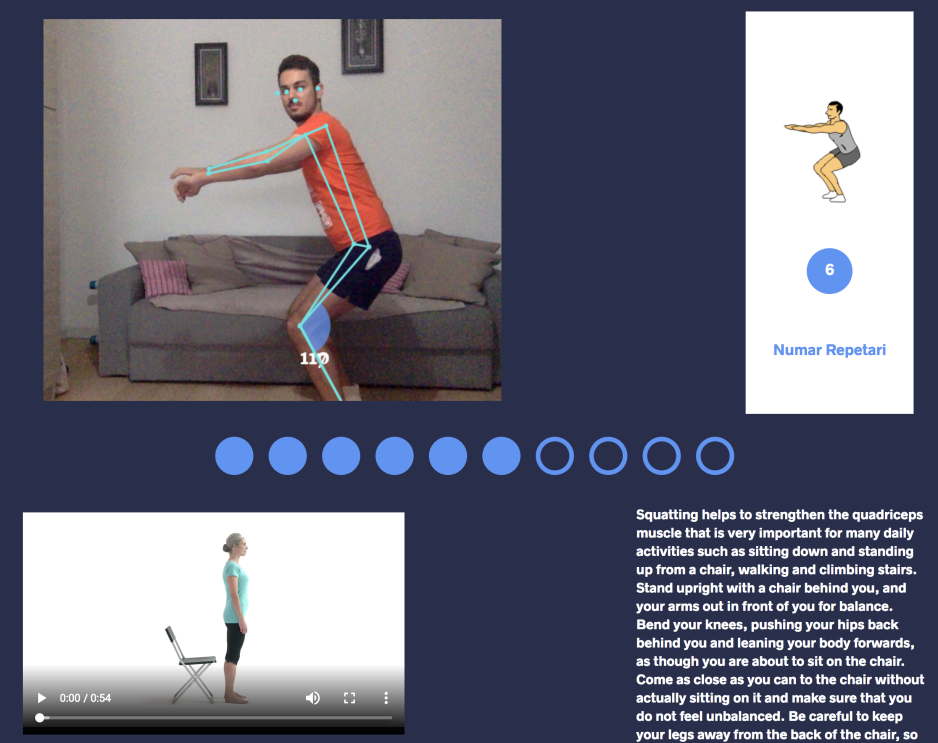
\includegraphics[scale=0.8]{fig/demo-mykineto.png}}  
	\caption{Demo of My Kineto}
\end{figure}

\section{Application development}
\subsection{Specification of the problem}
\subsection{Analysis and design}
\subsection{Implementation}
\subsection{Posture tracking algorithm}

\subsubsection{Initialization}
Initialization is the first part of the pose tracking algorithm, where we detect the posture with posenet and for each part of the detected skelet we calculate a bounding box and detect the initial set of keypoints that we are going to track in the next steps.
\subsubsection{Processing}
Processing is composed from three main parts: 
\begin{itemize}
    \item Tracking 
    \item Add new points 
    \item Respawn / Reinitialization
\end{itemize}
This part is used to track as much as possible points detected in the first phase.

\subsubsection{Keypoints tracking}
\par Points detected in the first part will be used inside tracking algorithm Lucas-Kanade \cite{Lucas:1981:IIR:1623264.1623280} (function calcOpticalFlowPyrLK() from OpenCV). This algorithm fits into the Detect Track  class (DT) and makes a local search to determine the new position of the points of interest detected in the previous frame. For this algorithm to work fine, it's important to take consecutive frames that are easily modified. If we do a sudden move, this algorithm will fail to detect to detect the new position of a part or even all the points in the previous frame. For this case, the next two steps in the algorithm will try to restore the system. 
\par The points in the system that are tracked are detected with Shi-Tomasi "Good features to track" \cite{323798}. 
\par After we detect new position for our keypoints we have to detect the new bounding box that correspond to their new position. For this task we choose to detect the homography matrix based on old points and new points position. Based on homography matrix we calculate the perspective transformation of previous bounding box.
\subsubsection{Add new points}
\par Adding new points is a step for restoring the system. As we track certain points, we may lose track of some of them. In this case, to prevent destabilization of the system, we will add new key points.
\par The system starts with a maximum number of key points. If a percentage of N of the maximum number of points is lost, then we will try to find others to replace the missing ones. 
\par The detection of new points will be achieved with the Shi-Tomasi algorithm "Good features to track". To narrow the search space of these algorithms, their implementations in OpenCV allow the definition of a mask. \par A mask is an image size matrix in which we want to find the key points. To mark the fact that we want to search in a certain area we will set the value of 1, the mask, in that region and 0 in the rest. Applying a mask is important not only to narrow the search space but also to don\mbox{'}t keep the points detected in an area where our posture skeleton is not found. 
\par More specifically in our application, for each bounding box built from the skelet we will add new points inside it. The calculated bounding box is used to create a mask that we can use inside the keypoints detection algorithm.
\subsubsection{Respawn / Reinitialization}
\par System reinitialization consists in the identification of the fact that we lost almost all of the tracked points and we are no longer able to estimate, with the remaining number of points, the skeleton posture. The algorithms used to reinitialize the posture are the ones used in the first phase. So basically from this phase if we are no longer able to track and estimate new posture of our skeleton then we go the the first step (Initialization).

\par System reinitialization denotes that the system has been completely destabilized. Loss of a large number of points can occur either due to a sudden movement or because the tracking posture is no longer in the frame.

\begin{figure}
	\centerline{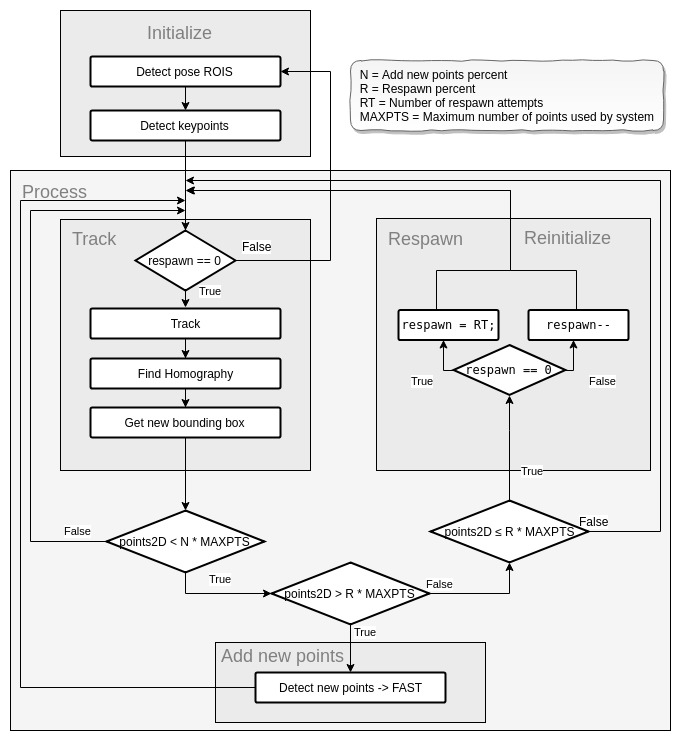
\includegraphics[scale=0.5]{fig/posture-tracking-algorithm.jpg}}  
	\caption{Posture tracking algorithm}
\end{figure}
\subsection{User manual}

\section{Experimental results and comparisons with similar approaches}

\section{Possible extensions}